\documentclass[12pt]{article}
\usepackage[table]{xcolor}
\usepackage[shortlabels]{enumitem}
\usepackage{tabularx,xltabular}
\usepackage{graphicx}
\usepackage{hyperref}
\usepackage{verbatim}
\usepackage{geometry}
\usepackage{ulem}
\usepackage[official]{eurosym}
\usepackage{tikz}
\usetikzlibrary{arrows,backgrounds,calc,decorations.markings,patterns,3d}
\usepackage{pgfplots}
\pgfplotsset{compat = newest}
\usetikzlibrary{fit}
\newcommand\addvmargin[1]{
\usetikzlibrary{arrows}
\node[fit=(current bounding box),inner ysep=#1,inner xsep=0]{};}
\usepackage{cancel}
\usepackage{fontspec}
\usepackage{array}  
\geometry{a4paper, top=2cm, left=2cm, right=2cm, bottom=2cm, headsep=1cm}
\usepackage{tabu}
\usepackage{pst-node}
\usepackage{colortbl}
\usepackage{array}
\usepackage{german}
\setlength\parindent{0pt}
\newcolumntype{?}{!{\vrule width 1pt}}
\usepackage{makecell}
\renewcommand{\arraystretch}{2.5}
\usepackage{pbox}
\usepackage{amssymb}
\usepackage{amsmath}
\usepackage{booktabs}
\newcolumntype{L}[1]{>{\raggedright\let\newline\\\arraybackslash\hspace{0pt}}m{#1}}
\newcolumntype{C}[1]{>{\centering\let\newline\\\arraybackslash\hspace{0pt}}m{#1}}
\newcolumntype{R}[1]{>{\raggedleft\let\newline\\\arraybackslash\hspace{0pt}}m{#1}}
\begin{document}
\rightline{Datum: 12.06.2023}
\centerline{{\Large Tägliche Übungen}} 
\vspace{1cm}
\noindent \\


\begin{xltabular}{\textwidth}{|C{0.75cm}|X|C{0.75cm}|X|}
\arrayrulecolor{black}\hline
a)&$-5-3+4\cdot b+4\cdot b=48$
&
b)&$3\cdot a-1+5\cdot a-1=46$
\\\hline
c)&$-3\cdot x+2-11+10\cdot x=61$
&
d)&$3-11+4\cdot a+5\cdot a=91$
\\\hline
\end{xltabular}
\vspace{0.5cm}
\noindent\tikzstyle{background grid}=[draw, black!30,step=.5cm]
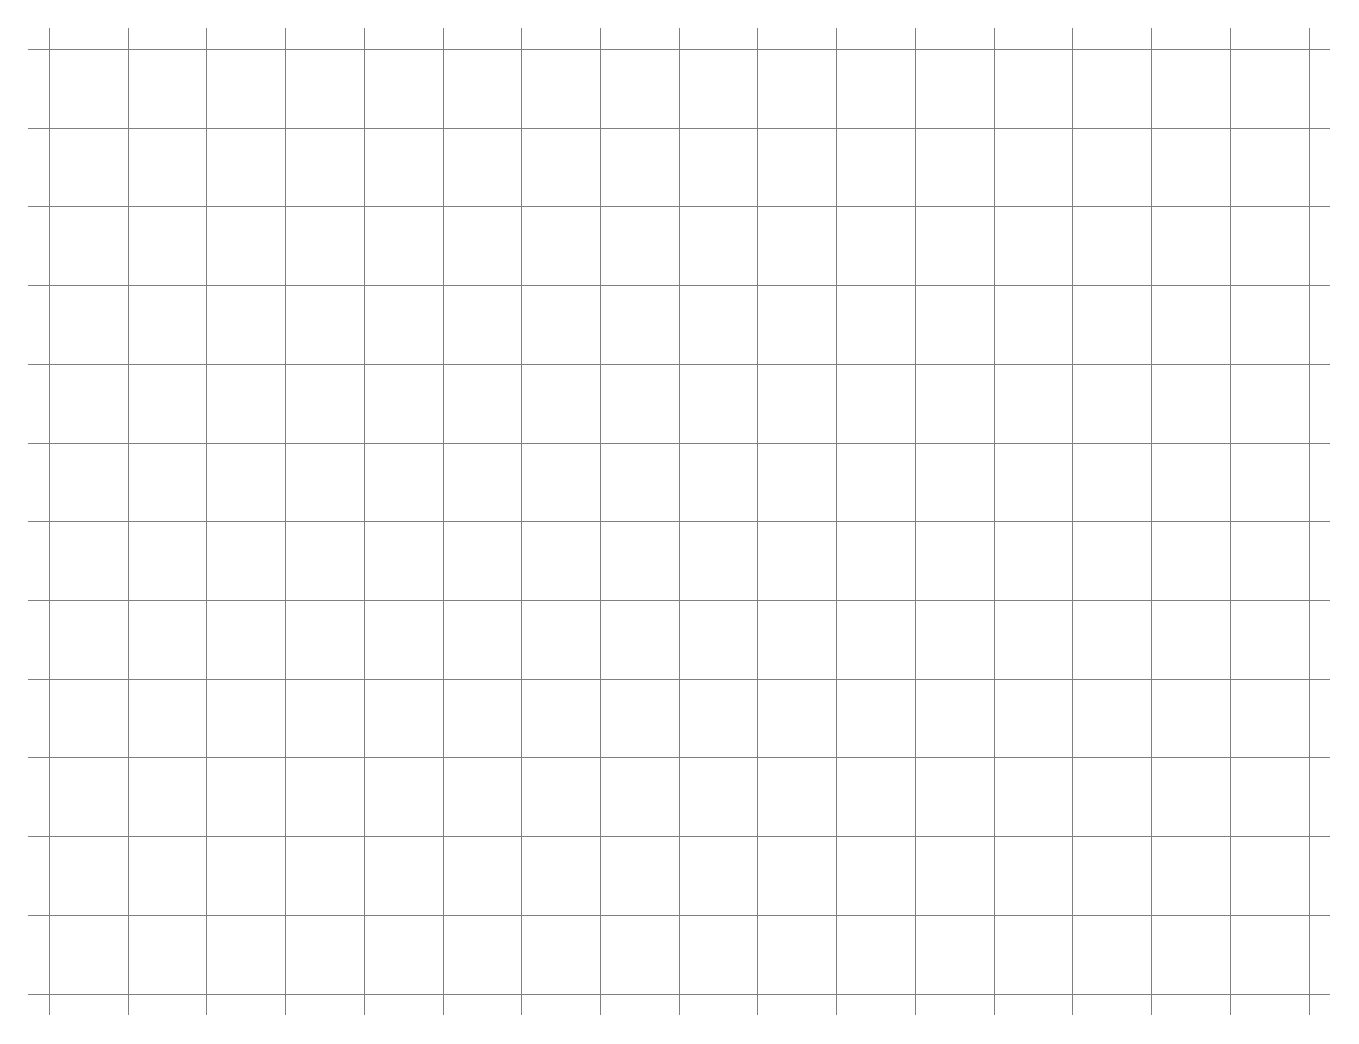
\begin{tikzpicture}[show background grid]
\node[] at (0,0) {};
\node[] at (16,12) {};
\end{tikzpicture}
\\
\newpage
\rightline{Datum: 12.06.2023}
\centerline{{\large Lösungen Tägliche Übungen}} 
\vspace{0.5cm}

\begin{xltabular}{\textwidth}{|C{0.75cm}|X|}
\arrayrulecolor{black}\hline
a)&\begingroup\setlength{\jot}{-0.03cm}
\tikzstyle{background grid}=[draw, black!15,step=.5cm]
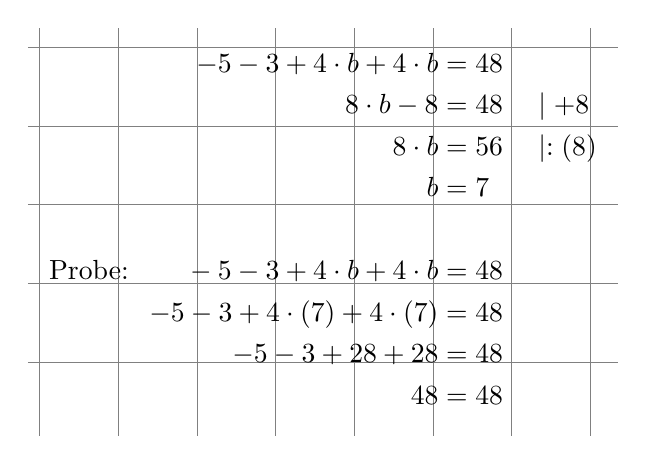
\begin{tikzpicture}[show background grid]
\node[below right] at (0,0.1) {
$\begin{aligned}
-5-3+4\cdot b+4\cdot b &=48& &  \\
8\cdot b - 8 &=48& & \mid + 8\\
8\cdot b &=56& & \mid :\left(8\right)\\
b &=7& & 
\\
\\
\mbox{Probe:}\qquad -5-3+4\cdot b+4\cdot b &=48& &  \\
-5-3+4\cdot \left(7\right)+4\cdot \left(7\right) &=48& &  \\
-5-3+28+28 &=48& &  \\
48 &=48& &  \\
\end{aligned}$};
\end{tikzpicture}
\endgroup
\\\hline
b)&\begingroup\setlength{\jot}{-0.03cm}
\tikzstyle{background grid}=[draw, black!15,step=.5cm]
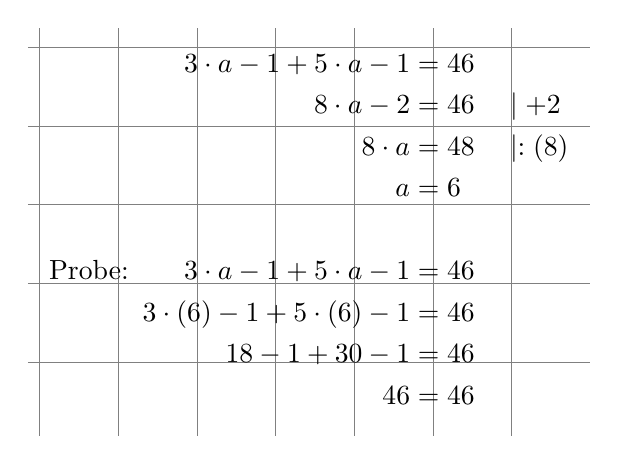
\begin{tikzpicture}[show background grid]
\node[below right] at (0,0.1) {
$\begin{aligned}
3\cdot a-1+5\cdot a-1 &=46& &  \\
8\cdot a - 2 &=46& & \mid + 2\\
8\cdot a &=48& & \mid :\left(8\right)\\
a &=6& & 
\\
\\
\mbox{Probe:}\qquad 3\cdot a-1+5\cdot a-1 &=46& &  \\
3\cdot \left(6\right)-1+5\cdot \left(6\right)-1 &=46& &  \\
18-1+30-1 &=46& &  \\
46 &=46& &  \\
\end{aligned}$};
\end{tikzpicture}
\endgroup
\\\hline
c)&\begingroup\setlength{\jot}{-0.03cm}
\tikzstyle{background grid}=[draw, black!15,step=.5cm]
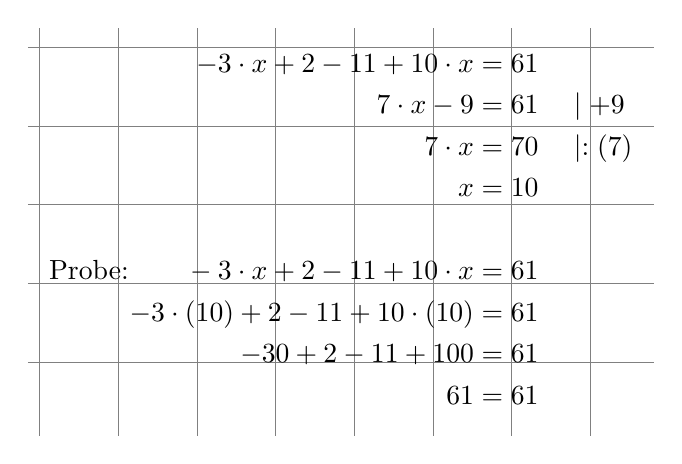
\begin{tikzpicture}[show background grid]
\node[below right] at (0,0.1) {
$\begin{aligned}
-3\cdot x+2-11+10\cdot x &=61& &  \\
7\cdot x - 9 &=61& & \mid + 9\\
7\cdot x &=70& & \mid :\left(7\right)\\
x &=10& & 
\\
\\
\mbox{Probe:}\qquad -3\cdot x+2-11+10\cdot x &=61& &  \\
-3\cdot \left(10\right)+2-11+10\cdot \left(10\right) &=61& &  \\
-30+2-11+100 &=61& &  \\
61 &=61& &  \\
\end{aligned}$};
\end{tikzpicture}
\endgroup
\\\hline
d)&\begingroup\setlength{\jot}{-0.03cm}
\tikzstyle{background grid}=[draw, black!15,step=.5cm]
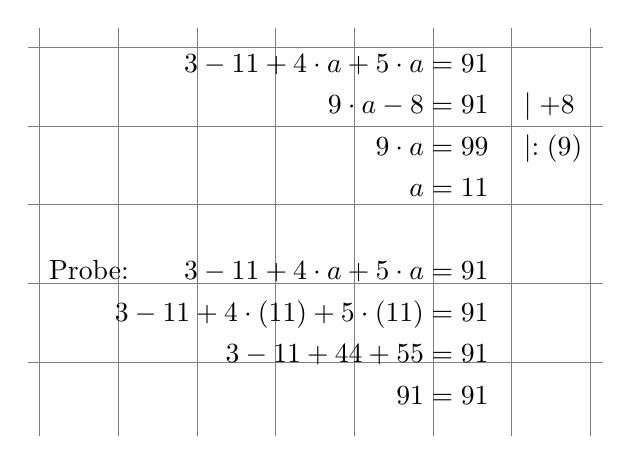
\begin{tikzpicture}[show background grid]
\node[below right] at (0,0.1) {
$\begin{aligned}
3-11+4\cdot a+5\cdot a &=91& &  \\
9\cdot a - 8 &=91& & \mid + 8\\
9\cdot a &=99& & \mid :\left(9\right)\\
a &=11& & 
\\
\\
\mbox{Probe:}\qquad 3-11+4\cdot a+5\cdot a &=91& &  \\
3-11+4\cdot \left(11\right)+5\cdot \left(11\right) &=91& &  \\
3-11+44+55 &=91& &  \\
91 &=91& &  \\
\end{aligned}$};
\end{tikzpicture}
\endgroup
\\\hline
\end{xltabular}
\vspace{0.5cm}
\end{document}